
\documentclass[11pt]{article} % use larger type; default would be 10pt
\usepackage{framed}
\usepackage[utf8]{inputenc} % set input encoding (not needed with XeLaTeX)
\usepackage{geometry} % to change the page dimensions
\geometry{a4paper} % or letterpaper (US) or a5paper or....
% \geometry{margin=2in} % for example, change the margins to 2 inches all round
% \geometry{landscape} % set up the page for landscape
%   read geometry.pdf for detailed page layout information

\usepackage{graphicx} % support the \includegraphics command and options

% \usepackage[parfill]{parskip} % Activate to begin paragraphs with an empty line rather than an indent

%%% PACKAGES
\usepackage{booktabs} % for much better looking tables
\usepackage{array} % for better arrays (eg matrices) in maths
\usepackage{paralist} % very flexible & customisable lists (eg. enumerate/itemize, etc.)
\usepackage{verbatim} % adds environment for commenting out blocks of text & for better verbatim
\usepackage{subfig} % make it possible to include more than one captioned figure/table in a single float
% These packages are all incorporated in the memoir class to one degree or another...
\usepackage{framed}

%%% HEADERS & FOOTERS
\usepackage{fancyhdr} % This should be set AFTER setting up the page geometry
\pagestyle{fancy} % options: empty , plain , fancy
\renewcommand{\headrulewidth}{0pt} % customise the layout...
\lhead{}\chead{}\rhead{}
\lfoot{}\cfoot{\thepage}\rfoot{}

%%% SECTION TITLE APPEARANCE
\usepackage{sectsty}
\allsectionsfont{\sffamily\mdseries\upshape} % (See the fntguide.pdf for font help)
% (This matches ConTeXt defaults)

%%% ToC (table of contents) APPEARANCE
\usepackage[nottoc,notlof,notlot]{tocbibind} % Put the bibliography in the ToC
\usepackage[titles,subfigure]{tocloft} % Alter the style of the Table of Contents
\renewcommand{\cftsecfont}{\rmfamily\mdseries\upshape}
\renewcommand{\cftsecpagefont}{\rmfamily\mdseries\upshape} % No bold!
\begin{document}
	

\section*{Week 7 Support Vector Machines}


%===================================================================%
\subsection*{Question 1}
Suppose you have trained an SVM classifier with a Gaussian kernel, and it learned the following decision boundary on the training set:
\begin{figure}[h!]
\centering
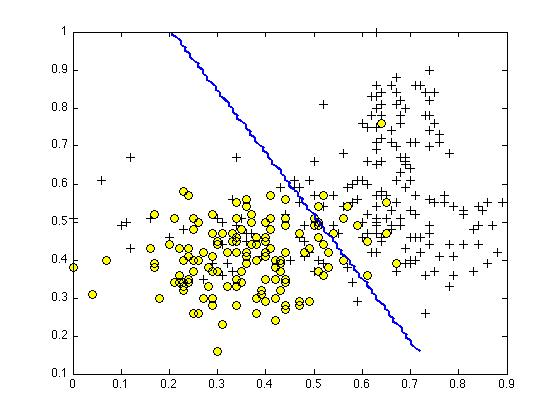
\includegraphics[width=0.7\linewidth]{images/SVM1}
\end{figure}


You suspect that the SVM is underfitting your dataset. Should you try increasing or decreasing C? Increasing or decreasing $\sigma^2$?

\begin{itemize}
	\item It would be reasonable to try decreasing C. It would also be reasonable to try decreasing $\sigma^2$.
	
	\item \textbf{CORRECT} It would be reasonable to try increasing C. It would also be reasonable to try decreasing $\sigma^2$.
	
	\item It would be reasonable to try increasing C. It would also be reasonable to try increasing $\sigma^2$.
	
	\item It would be reasonable to try decreasing C. It would also be reasonable to try increasing $\sigma^2$.
\end{itemize}


%===================================================================%
\newpage
\subsection*{Question 2}
The formula for the Gaussian kernel is given by % similarity(x,l(1))=exp(−||x−l(1)||22σ2) .
\begin{figure}[h!]
\centering
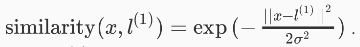
\includegraphics[width=0.5\linewidth]{images/SVM-Similarity}

\end{figure}

The figure below shows a plot of $f_1$=similarity(x,l(1)) when $\sigma^2 = 1$.

\begin{figure}[h!]
	\centering
	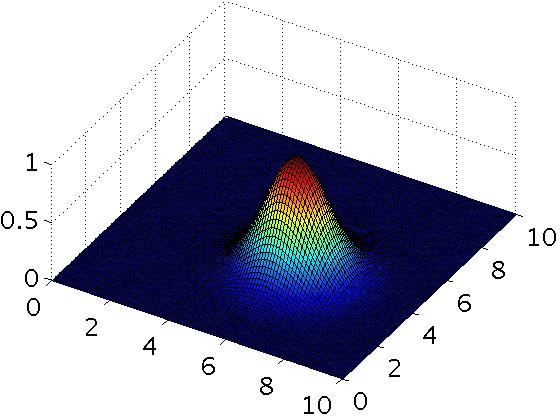
\includegraphics[width=0.5\linewidth]{images/SVM2}
\end{figure}
\newpage
\subsubsection*{Options}
Which of the following is a plot of f1 when $\sigma^2 = 0.25$?
\begin{figure}[h!]
		\centering
		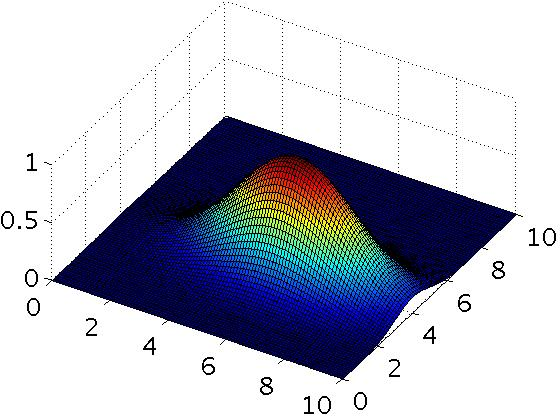
\includegraphics[width=0.4\linewidth]{images/SVM3}
	\caption{Option 1}
		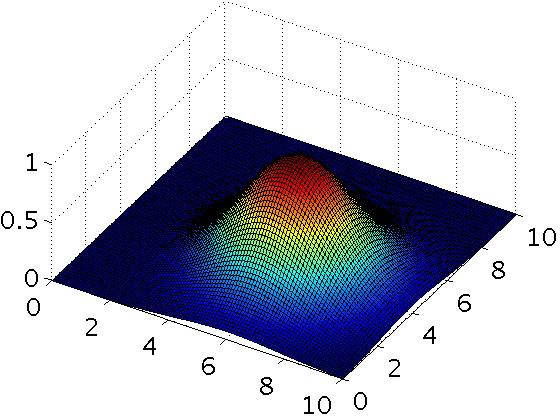
\includegraphics[width=0.4\linewidth]{images/SVM4}
	\caption{Option 2}
		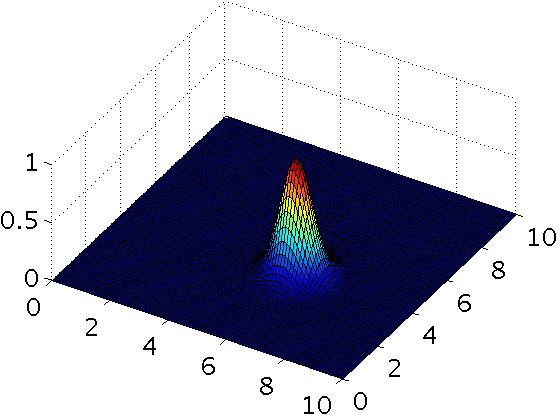
\includegraphics[width=0.4\linewidth]{images/SVM5}
		\caption{Option 3}		
\end{figure}
\newpage




%===================================================================%
\subsection*{Question 3}
\begin{figure}[h!]
\centering
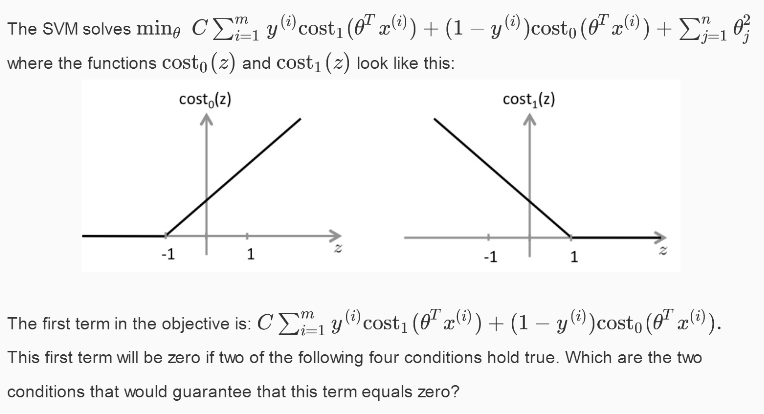
\includegraphics[width=01.1\linewidth]{images/SVM-costquestion}
\end{figure}


\begin{itemize}
\item For every example with y(i)=1, we have that $ \theta^T x(i)\geq 0$.

\item For every example with y(i)=0, we have that $ \theta^T x(i)\leq 0$.

\item CORRECT For every example with y(i)=1, we have that $ \theta^T x(i)\geq 1$.

\item CORRECT For every example with y(i)=0, we have that $ \theta^T x(i)\leq -1$.
\end{itemize}

%===================================================================%
\subsection*{Question 4}
Suppose you have a dataset with n = 10 features and m = 5000 examples.

After training your logistic regression classifier with gradient descent, you find that it has underfit the training set and does not achieve the desired performance on the training or cross validation sets.

Which of the following might be promising steps to take? Check all that apply.
\begin{itemize}
	\item CORRECT Try using a neural network with a large number of hidden units.
	
	\item WRONG Use a different optimization method since using gradient descent to train logistic regression might result in a local minimum.
	
	\item Reduce the number of examples in the training set.
	
	\item CORRECT Create / add new polynomial features.
\end{itemize}


%===================================================================%
\subsection*{Question 5} 
Which of the following statements are true? Check all that apply.

\begin{itemize}
	\item If the data are linearly separable, an SVM using a linear kernel will return the same parameters $\theta$ regardless of the chosen value of
	C (i.e., the resulting value of $\theta$ does not depend on C).
	
	\item CORRECT It is important to perform feature normalization before using the Gaussian kernel.
	
	\item Suppose you are using SVMs to do multi-class classification and 	would like to use the one-vs-all approach. If you have K differentclasses, you will train K - 1 different SVMs.
	
	\item CORRECT The maximum value of the Gaussian kernel (i.e., sim(x,l(1))) is 1.
\end{itemize}


%=====================================================================================%



\end{document}
